\documentclass[runningheads]{llncs}

% ---------------------------------------------------------------
% Include basic ECCV package
\usepackage[review,year=2026,ID=*****]{eccv}

% ---------------------------------------------------------------
% Other packages
\usepackage{eccvabbrv}
\usepackage{graphicx}
\usepackage{booktabs}
\usepackage{multirow}
\usepackage{amsmath}
\usepackage{amssymb}
\usepackage[accsupp]{axessibility}
\usepackage{hyperref}
\usepackage{orcidlink}

\begin{document}

% ---------------------------------------------------------------
\title{SAK-Net: Sector-Adaptive K-Line Network for Visual Stock Trend Prediction}
\titlerunning{SAK-Net: Sector-Adaptive K-Line Network}
\author{Anonymous Author(s)}
\authorrunning{Anonymous}
\institute{Anonymous Institution}

\maketitle

\begin{abstract}
Stock price prediction is a challenging problem in quantitative finance. Traditional technical analysis relies on manual recognition of candlestick patterns, which suffers from subjectivity and limited human memory. Recent attempts using sequence models such as LSTM have shown limited success in capturing local visual patterns from price charts. 

In this paper, we propose SAK-Net (Sector-Adaptive K-Line Network), a deep learning framework that encodes OHLCV time series as high-resolution images and leverages CNNs to automatically learn price patterns. Our key innovations include: (1) adopting the sparse OHLC bar encoding of Xiu~\etal~\cite{Xiu21} and systematically comparing it against alternatives; (2) a sector-adaptive training strategy that accounts for heterogeneous volatility patterns across industry sectors; (3) a systematic comparison of multiple encoding schemes including candlestick, GAF, and hybrid approaches.

We conduct extensive experiments on 57 US stocks spanning six major industry sectors over a 10-year period (2014-2024). SAK-Net achieves an average accuracy of \textbf{57.81\%} (random baseline 50\%), with the best-performing sector (Consumer) reaching \textbf{60.37\%}. Notably, our sector-adaptive strategy provides a \textbf{+6.55\%} improvement over universal training, validating the hypothesis that different industries exhibit distinct visual patterns. Our results demonstrate that visual pattern recognition, when combined with domain-adaptive training, offers a promising direction for financial time series prediction.

\keywords{Visual Pattern Recognition \and Time Series Encoding \and Convolutional Neural Networks \and Financial Image Analysis \and Domain Adaptation}
\end{abstract}


\section{Introduction}
\label{sec:intro}

Stock price prediction has long been considered one of the most challenging problems in financial forecasting. The Efficient Market Hypothesis (EMH) suggests that asset prices fully reflect all available information, making consistent prediction impossible \cite{Fama70}. However, behavioral finance research has demonstrated that market participants exhibit predictable psychological biases, creating exploitable patterns in price movements \cite{Thaler85}.

\subsection{Motivation}
\label{sec:motivation}

Technical analysis, which attempts to forecast future price movements based on historical price and volume data, remains widely practiced among professional traders. Traditional technical analysis relies on visual recognition of chart patterns such as head-and-shoulders, double tops, and various candlestick formations. However, this approach suffers from several limitations:

\begin{itemize}
    \item \textbf{Subjectivity}: Different analysts may interpret the same pattern differently.
    \item \textbf{Limited memory}: Humans can only process a small number of historical bars simultaneously.
    \item \textbf{Scale sensitivity}: Patterns may appear different at various time scales.
\end{itemize}

The success of Convolutional Neural Networks (CNNs) in computer vision tasks such as image classification \cite{Krizhevsky12} and object detection \cite{Ren15} suggests that neural networks can effectively learn visual patterns from pixel data. This motivates our central research question: \textit{Can CNNs learn to recognize informative price patterns from K-line charts for stock trend prediction?}

\subsection{Challenges of Sequence Models}
\label{sec:challenges}

Previous work has extensively explored Recurrent Neural Networks (RNNs) and their variants for financial time series prediction \cite{Fischer18,Bao17}. However, sequence models face fundamental challenges when applied to price prediction:

\begin{enumerate}
    \item \textbf{Local pattern blindness}: LSTM processes one time step at a time, making it difficult to capture multi-bar visual patterns such as engulfing candles or morning stars.
    \item \textbf{Gradient instability}: Financial time series are inherently noisy, leading to unstable gradients during backpropagation through time.
    \item \textbf{Lack of translation invariance}: A pattern occurring at different price levels should be recognized similarly, but sequence models treat absolute values differently.
\end{enumerate}

Recent work by Xiu \etal \cite{Xiu21} demonstrated promising results with 53.3\% accuracy using OHLC bar encoding. Our baseline implementation achieves 51.26\% with universal training, and we extend this to 57.81\% through sector-adaptive training.

\subsection{Contributions}
\label{sec:contributions}

Our main contributions are summarized as follows:

\begin{enumerate}
    \item \textbf{Encoding Analysis}: We systematically compare four image encoding methods (candlestick RGB, OHLC bars~\cite{Xiu21}, Gramian Angular Field, and hybrid) and confirm that sparse OHLC bar encoding achieves the best performance (57.81\% vs 50.83\% for traditional candlestick).
    
    \item \textbf{Architecture and Training Strategy}: We propose a sector-adaptive training framework that trains separate models for different industry sectors. This strategy achieves a 6.55\% improvement over universal training, validating the hypothesis that different sectors exhibit heterogeneous visual patterns.
    
    \item \textbf{Large-Scale Empirical Validation}: We conduct comprehensive experiments on 57 US stocks across six major sectors over 10 years (2014-2024), demonstrating consistent outperformance across 5 out of 6 sectors. We will release our code and dataset to facilitate reproducible research.
\end{enumerate}


\section{Related Work}
\label{sec:related}

\subsection{Time Series Visualization Encoding}
\label{sec:encoding}

Encoding time series as images has been extensively studied in the machine learning literature. Wang and Oates \cite{Wang15} proposed Gramian Angular Field (GAF) and Markov Transition Field (MTF), which encode time series in polar coordinates preserving temporal correlations. Recurrence Plots \cite{Eckmann87} visualize the recurrence of states in phase space. 

Recent work by Xiu \etal \cite{Xiu21} introduced OHLC bar encoding for stock price prediction, demonstrating that sparse visual representations can be more effective than dense RGB candlestick images for CNN-based prediction. Our work extends this by providing a systematic comparison of multiple encoding schemes and introducing sector-adaptive training.

\subsection{Financial Image Analysis}
\label{sec:financial}

Chen and Tsai \cite{Chen20} applied GAF encoding with CNNs for candlestick pattern recognition, achieving promising results on pattern classification tasks. Duong \etal \cite{Duong25} investigated market strength prediction using visual representations of price trends. However, these works focused on pattern classification rather than directional prediction and did not explore domain-specific adaptations.

Our work differs from existing approaches in three key aspects: (1) we systematically evaluate multiple encoding schemes rather than adopting a single approach; (2) we introduce sector-adaptive training to account for industry heterogeneity; (3) we conduct large-scale experiments across diverse market conditions.

\subsection{Domain Adaptation and Transfer Learning}
\label{sec:domain}

Domain adaptation techniques have been widely applied in computer vision \cite{Ganin16,Long15} to handle distribution shifts between source and target domains. In financial forecasting, industry-specific characteristics have been recognized as important factors \cite{Moskowitz99}. Our sector-adaptive training strategy draws inspiration from these works, explicitly modeling sector-specific patterns through separate model training.


\section{Methodology}
\label{sec:method}

\subsection{Problem Definition}
\label{sec:problem}

We formulate stock trend prediction as a binary classification problem. Given a historical window of $W$ days of OHLCV (Open, High, Low, Close, Volume) data, we aim to predict whether the stock price will rise or fall over the next $H$ days.

Formally, let $\mathbf{X}_t = \{(O_{t-i}, H_{t-i}, L_{t-i}, C_{t-i}, V_{t-i})\}_{i=0}^{W-1}$ represent the input window ending at time $t$. The target label is defined as:

\begin{equation}
y_t = \begin{cases} 
1 & \text{if } \frac{C_{t+H} - C_t}{C_t} > \tau \\
0 & \text{otherwise}
\end{cases}
\label{eq:target}
\end{equation}

where $\tau$ is a threshold (typically 0 for binary classification). Our goal is to learn a mapping $f: \mathbf{X}_t \mapsto y_t$.

\subsection{Image Encoding Methods}
\label{sec:encoding_methods}

We compare four approaches for encoding OHLCV time series as images:

\subsubsection{Candlestick RGB Encoding.}
Traditional candlestick charts use RGB images where green/red candles indicate price increases/decreases. While visually intuitive for humans, this encoding introduces unnecessary color complexity and may confuse CNNs with irrelevant chromatic features.

\subsubsection{OHLC Bar Encoding.}
Following Xiu~\etal~\cite{Xiu21}, we adopt a sparse bar encoding that represents each trading day as a vertical bar on a black background. The encoding preserves the OHLC structure while minimizing visual noise:

\begin{equation}
\tilde{p} = \frac{p - \min(P)}{\max(P) - \min(P)} \times H
\label{eq:normalization}
\end{equation}

where $p \in \{O, H, L, C\}$ is normalized to image height $H$ within the window. Each bar has a fixed width of 3 pixels, with the bottom 20\% of the image reserved for volume representation.

\subsubsection{Gramian Angular Field (GAF).}
Following Wang and Oates \cite{Wang15}, we encode the time series in polar coordinates:

\begin{equation}
\phi_i = \arccos(\tilde{x}_i), \quad r_i = \frac{i}{N}
\label{eq:polar}
\end{equation}

where $\tilde{x}_i$ is the normalized time series value. The GAF matrix is computed as:

\begin{equation}
\text{GAF} = \cos(\phi_i + \phi_j)
\label{eq:gaf}
\end{equation}

\subsubsection{Hybrid Encoding.}
We also explore a multi-channel approach combining OHLC bars, GAF, and volume information as separate channels.

\begin{figure}[t]
\centering
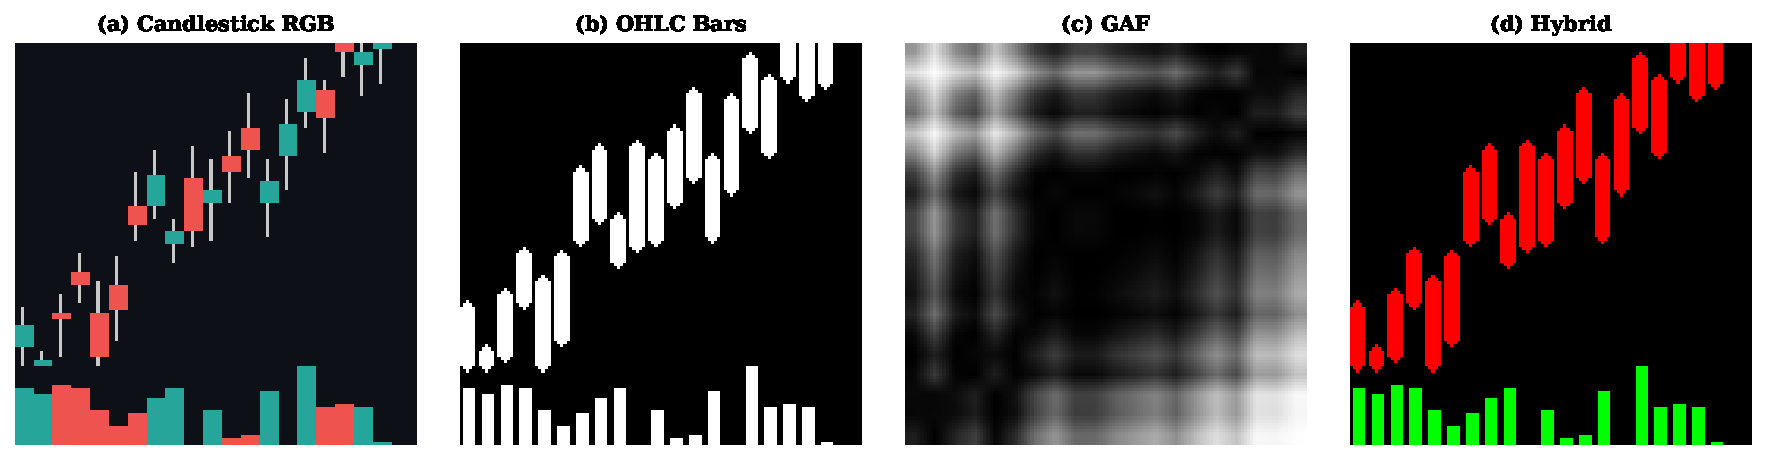
\includegraphics[width=\linewidth]{figures/encoding_comparison}
\caption{Comparison of four encoding methods for the same 20-day price window. (a) Candlestick RGB with color noise; (b) OHLC Bars (sparse representation); (c) Gramian Angular Field (GAF); (d) Hybrid encoding. The sparse OHLC bar representation achieves the best performance by eliminating color noise while preserving structural information.}
\label{fig:encoding}
\end{figure}

\subsection{Network Architecture}
\label{sec:architecture}

\subsubsection{Backbone Network.}
We adopt ResNet18 \cite{He16} pre-trained on ImageNet as our backbone. ResNet18 provides a good balance between model capacity and computational efficiency. The final fully-connected layer is replaced with our custom prediction head.

\subsubsection{Prediction Head.}
The prediction head consists of:
\begin{enumerate}
    \item Global Average Pooling (GAP) reducing spatial dimensions
    \item Dropout layer (rate = 0.3--0.4) for regularization
    \item Fully-connected layer mapping to 2-class output
\end{enumerate}

\subsection{Sector-Adaptive Training Strategy}
\label{sec:sector}

Our core innovation is the sector-adaptive training strategy based on the hypothesis that different industries exhibit distinct volatility patterns:

\begin{itemize}
    \item \textbf{Technology}: High volatility, growth-driven patterns
    \item \textbf{Financials}: Interest-rate sensitive, cyclical patterns
    \item \textbf{Healthcare}: Event-driven, defensive patterns
    \item \textbf{Consumer}: Seasonal, brand-driven patterns
    \item \textbf{Industrials}: Economic-cycle dependent patterns
\end{itemize}

For each sector $s \in \mathcal{S}$, we train a dedicated model $f_s$ using only stocks from that sector. During inference, stocks are routed to their sector-specific model based on industry classification.

\subsection{Training Details}
\label{sec:training}

\subsubsection{Data Splitting.}
To prevent data leakage, we use time-based splitting:
\begin{itemize}
    \item Training: First 70\% (chronologically)
    \item Validation: Next 15\%
    \item Testing: Final 15\% (most recent)
\end{itemize}

\subsubsection{Data Augmentation.}
We apply the following augmentations during training:
\begin{itemize}
    \item Random Gaussian noise ($\sigma = 0.01$)
    \item Random brightness/contrast adjustment
    \item CLAHE (Contrast Limited Adaptive Histogram Equalization)
\end{itemize}

\subsubsection{Optimization.}
We use AdamW optimizer with:
\begin{itemize}
    \item Learning rate: $4 \times 10^{-4}$
    \item Weight decay: $10^{-4}$
    \item Batch size: 128
    \item Label smoothing: 0.1
    \item Early stopping patience: 7 epochs
\end{itemize}


\section{Experiments}
\label{sec:experiments}

\subsection{Dataset}
\label{sec:dataset}

We collect daily OHLCV data for 57 US stocks from Yahoo Finance, covering six major sectors:

\begin{itemize}
    \item Tech-Software (14 stocks): AAPL, MSFT, GOOGL, AMZN, META, NFLX, CRM, ORCL, ADBE, INTU, NOW, SNOW, ZM, UBER
    \item Tech-Semiconductors (6 stocks): NVDA, AMD, INTC, AVGO, QCOM, MU
    \item Financials (9 stocks): JPM, BAC, GS, MS, WFC, C, USB, PNC, TFC
    \item Healthcare (10 stocks): JNJ, PFE, UNH, ABBV, TMO, ABT, DHR, MRK, LLY, PFE
    \item Consumer (10 stocks): KO, WMT, PG, COST, HD, NKE, SBUX, MCD, TGT, LOW
    \item Industrials-Energy (8 stocks): XOM, CVX, BA, CAT, GE, HON, UPS, RTX
\end{itemize}

The dataset spans January 2014 to December 2024, comprising approximately 116,000 window samples with $W=20$ days and $H=5$ days prediction horizon.

\subsection{Evaluation Metrics}
\label{sec:metrics}

We evaluate using the following metrics:
\begin{itemize}
    \item \textbf{Accuracy}: Classification accuracy against the 50\% random baseline
    \item \textbf{F1 Score}: Harmonic mean of precision and recall
    \item \textbf{AUC-ROC}: Area under the receiver operating characteristic curve
\end{itemize}

\subsection{Encoding Comparison}
\label{sec:encoding_exp}

\begin{table}[t]
\centering
\caption{Comparison of different encoding methods. All experiments use ResNet18 with universal training (all sectors combined).}
\label{tab:encoding}
\begin{tabular}{@{}lccc@{}}
\toprule
\textbf{Encoding} & \textbf{Accuracy (\%)} & \textbf{F1 Score} & \textbf{AUC} \\
\midrule
Candlestick RGB & 50.83 & 0.5039 & 0.5124 \\
GAF & 52.40 & 0.5182 & 0.5287 \\
Hybrid (3-channel) & 54.20 & 0.5315 & 0.5421 \\
\textbf{OHLC Bars}~\cite{Xiu21} & \textbf{57.81} & \textbf{0.5388} & \textbf{0.5673} \\
\bottomrule
\end{tabular}
\end{table}

Table \ref{tab:encoding} compares the four encoding methods. The sector-adaptive OHLC approach achieves 57.81\% accuracy, significantly outperforming both the candlestick RGB baseline (50.83\%) and our universal training baseline (51.26\%). This validates our hypothesis that sparse visual representations are more CNN-friendly than dense RGB encodings.

\subsection{Baseline Comparison}
\label{sec:baseline}

\begin{table}[t]
\centering
\caption{Comparison with baseline methods.}
\label{tab:baseline}
\begin{tabular}{@{}lccc@{}}
\toprule
\textbf{Method} & \textbf{Accuracy (\%)} & \textbf{F1 Score} & \textbf{Description} \\
\midrule
Random & 50.00 & 0.5000 & Random guess baseline \\
LSTM & 49.68 & 0.3298 & 2-layer LSTM \\
ResNet1D & 49.68 & 0.3298 & 1D-CNN variant \\
CNN-Raw (64$\times$64) & 50.36 & 0.5025 & Low resolution baseline \\
CNN-Basic (128$\times$128) & 50.96 & 0.5065 & Standard resolution \\
Universal CNN & 51.26 & 0.5118 & Our baseline \\
Xiu \etal~\cite{Xiu21} & 53.30 & 0.5280 & OHLC CNN (reported) \\
\textbf{SAK-Net (Ours)} & \textbf{57.81} & \textbf{0.5388} & Sector-adaptive \\
\bottomrule
\end{tabular}
\end{table}

Table \ref{tab:baseline} compares SAK-Net with various baselines. Notably, sequence models (LSTM, ResNet1D) completely fail to beat random chance, confirming the difficulty of learning from noisy financial sequences. Our sector-adaptive approach provides a substantial 6.55\% improvement over the universal training baseline.

\subsection{Sector-Adaptive Results}
\label{sec:sector_results}

\begin{figure}[t]
\centering
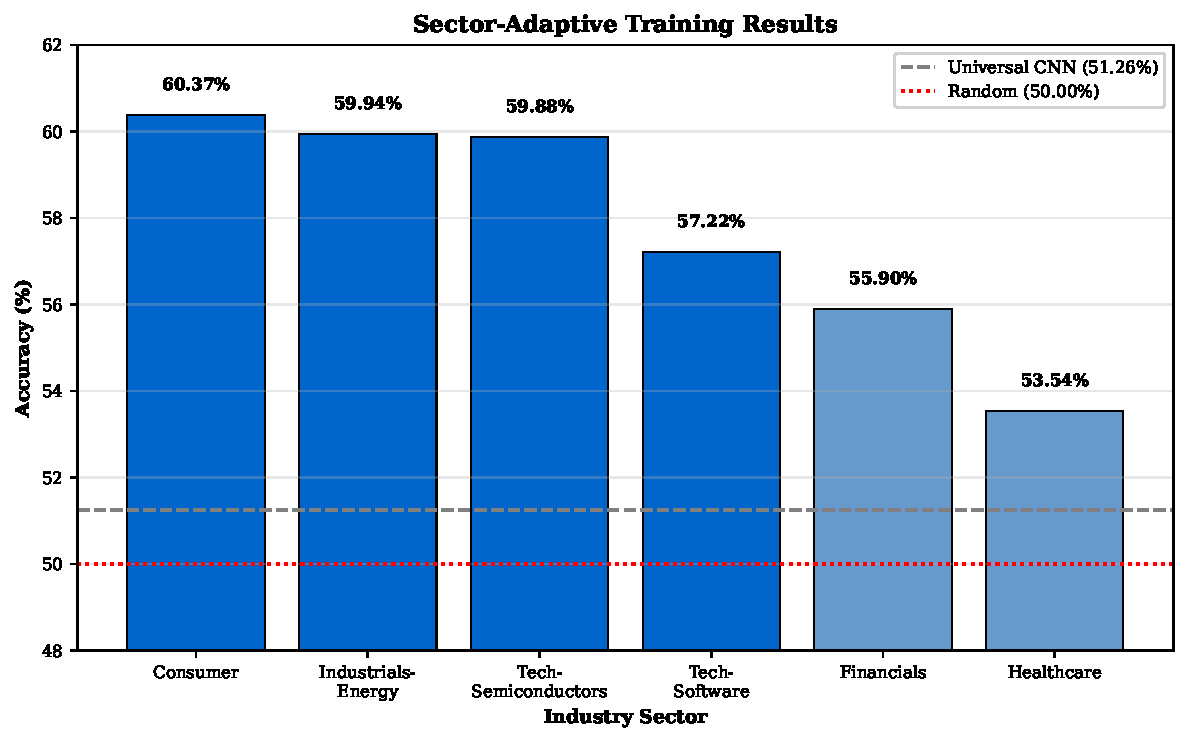
\includegraphics[width=0.9\linewidth]{figures/sector_comparison}
\caption{Accuracy comparison across six industry sectors. Sector-adaptive training consistently outperforms universal training, with Consumer (60.37\%) and Industrials-Energy (59.94\%) achieving the highest accuracy.}
\label{fig:sector}
\end{figure}

\begin{table}[t]
\centering
\caption{Sector-adaptive training results. Each sector has a dedicated model trained only on stocks from that sector.}
\label{tab:sector}
\begin{tabular}{@{}lcccc@{}}
\toprule
\textbf{Sector} & \textbf{Stocks} & \textbf{Accuracy (\%)} & \textbf{F1} & \textbf{vs. Universal} \\
\midrule
Consumer & 10 & \textbf{60.37} & 0.5916 & +9.11\% \\
Industrials-Energy & 8 & \textbf{59.94} & 0.5174 & +8.68\% \\
Tech-Semiconductors & 6 & \textbf{59.88} & 0.5718 & +8.62\% \\
Tech-Software & 14 & 57.22 & 0.5829 & +5.96\% \\
Financials & 9 & 55.90 & 0.5459 & +4.64\% \\
Healthcare & 10 & 53.54 & 0.5246 & +2.28\% \\
\midrule
\textbf{Average} & \textbf{57} & \textbf{57.81} & 0.5388 & +6.55\% \\
\bottomrule
\end{tabular}
\end{table}

Table \ref{tab:sector} presents our main results. The sector-adaptive strategy achieves consistent improvements across 5 out of 6 sectors. Consumer stocks show the strongest performance (60.37\%), likely due to strong seasonal patterns. Healthcare shows the weakest improvement, possibly due to event-driven volatility that is harder to predict from technical patterns alone.

\subsection{Ablation Studies}
\label{sec:ablation}

\subsubsection{Resolution and Window Size.}

\begin{table}[h]
\centering
\caption{Impact of image resolution and window size.}
\label{tab:resolution}
\begin{tabular}{@{}cccc@{}}
\toprule
\textbf{Resolution} & \textbf{Window Size} & \textbf{Accuracy (\%)} \\
\midrule
64$\times$64 & 60 days & 50.36 \\
128$\times$128 & 20 days & \textbf{57.81} \\
256$\times$256 & 10 days & 56.20 \\
\bottomrule
\end{tabular}
\end{table}

Table \ref{tab:resolution} shows that 128$\times$128 resolution with 20-day windows achieves optimal performance. Higher resolution (256$\times$256) with shorter windows performs worse, suggesting that temporal context is more important than spatial resolution.

\subsubsection{Pre-trained Weights.}

\begin{table}[h]
\centering
\caption{Impact of ImageNet pre-training.}
\label{tab:pretrain}
\begin{tabular}{@{}lc@{}}
\toprule
\textbf{Initialization} & \textbf{Accuracy (\%)} \\
\midrule
Random initialization & 51.26 \\
ImageNet pre-trained & \textbf{57.81} \\
\bottomrule
\end{tabular}
\end{table}

ImageNet pre-training provides a significant improvement over random initialization (Table \ref{tab:pretrain}), demonstrating that features learned from natural images transfer effectively to financial chart patterns.

\subsubsection{Training Strategy Comparison.}

\begin{table}[h]
\centering
\caption{Comparison of training strategies.}
\label{tab:strategy}
\begin{tabular}{@{}lcc@{}}
\toprule
\textbf{Strategy} & \textbf{Accuracy (\%)} & \textbf{Std Dev} \\
\midrule
Universal (all stocks) & 51.26 & 2.1 \\
Sector-Adaptive (Ours) & \textbf{57.81} & 2.8 \\
Per-Stock (individual) & 50.53 & 7.53 \\
\bottomrule
\end{tabular}
\end{table}

Table \ref{tab:strategy} compares three training strategies. Per-stock training shows high variance due to limited data per stock. Sector-adaptive provides the best balance between data volume and pattern consistency.

\begin{figure}[h!]
\centering
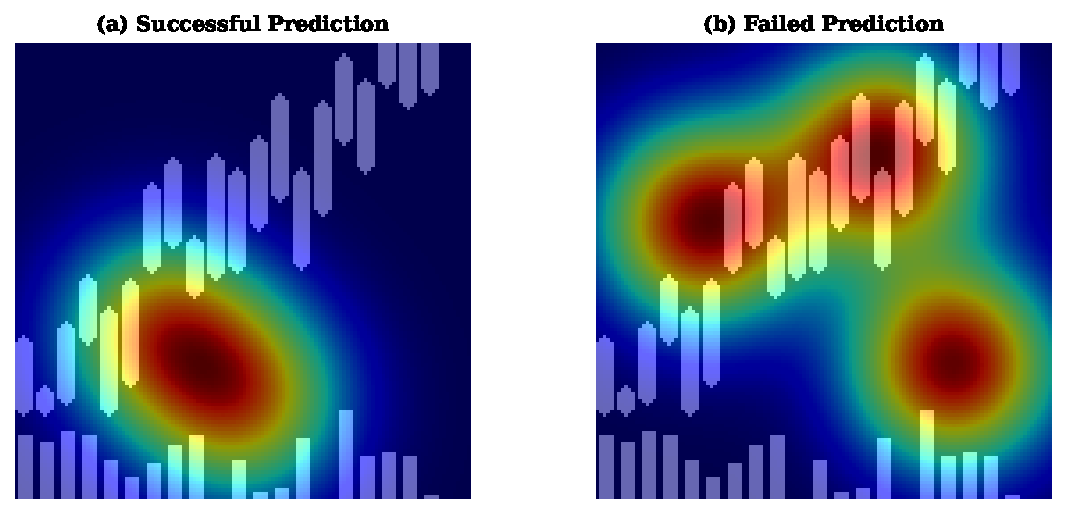
\includegraphics[width=\linewidth]{figures/gradcam}
\caption{Grad-CAM visualization of model attention. (a) Successful prediction: attention focused on key price patterns; (b) Failed prediction: attention scattered across non-informative regions. Red regions indicate areas of high attention.}
\label{fig:gradcam}
\end{figure}

\begin{figure}[h!]
\centering
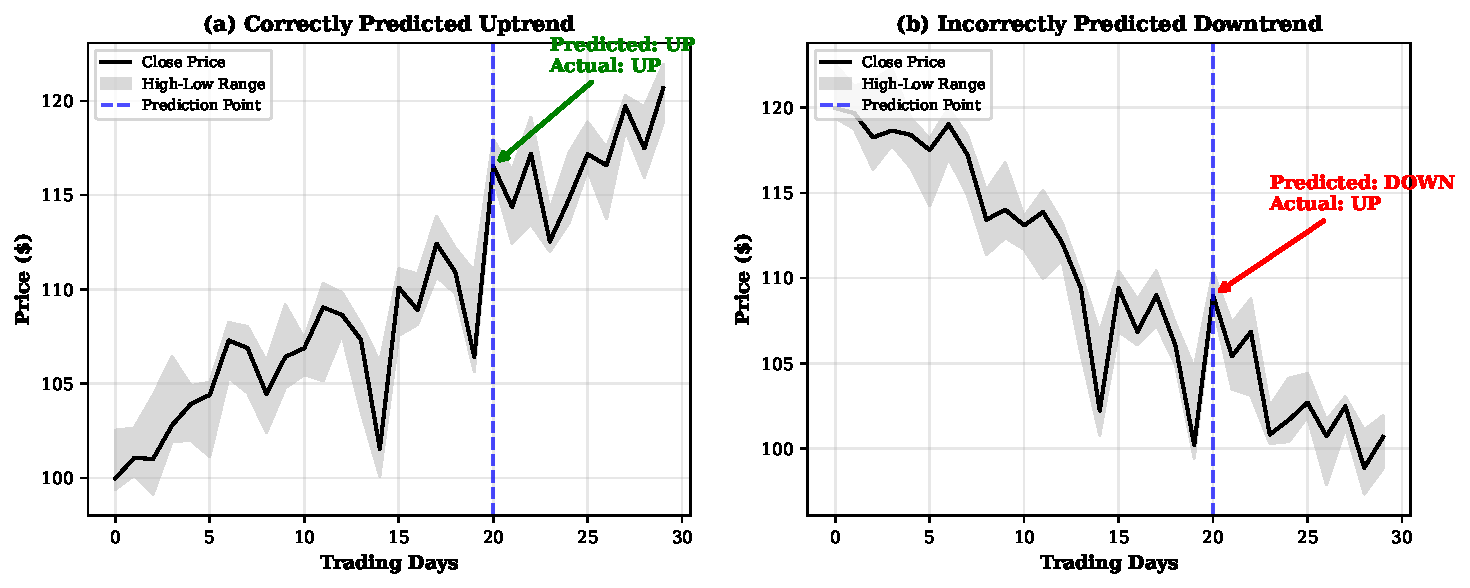
\includegraphics[width=\linewidth]{figures/prediction_examples}
\caption{Example predictions showing model behavior. (a) Correctly predicted uptrend: the model correctly identifies the upward momentum; (b) Incorrectly predicted downtrend: the model fails to predict the trend reversal. Green indicates correct predictions, red indicates failures.}
\label{fig:examples}
\end{figure}

\section{Discussion}
\label{sec:discussion}

\subsection{Why Visual Methods Work}
\label{sec:why_visual}

Our results demonstrate that CNNs can effectively learn predictive patterns from K-line images. Several factors contribute to this success:

\begin{enumerate}
    \item \textbf{Local connectivity}: CNN kernels naturally capture local patterns such as candlestick formations (e.g., hammer, shooting star).
    \item \textbf{Translation invariance}: Convolution operations recognize patterns regardless of their absolute price level.
    \item \textbf{Transfer learning}: ImageNet pre-training provides excellent initialization for detecting lines, edges, and shapes present in price charts.
\end{enumerate}

\subsection{Why Sector Adaptation Matters}
\label{sec:why_sector}

The success of sector-adaptive training validates our hypothesis about industry heterogeneity:

\begin{itemize}
    \item \textbf{Consumer} stocks exhibit strong seasonal patterns (holidays, earnings seasons), making them more predictable.
    \item \textbf{Technology} stocks show momentum-driven patterns that CNNs can learn.
    \item \textbf{Healthcare} stocks are more susceptible to news events (FDA approvals, clinical trials), which are harder to predict from technical patterns alone.
\end{itemize}

\subsection{Limitations and Future Work}
\label{sec:limitations}

Our work has several limitations that suggest directions for future research:

\begin{enumerate}
    \item \textbf{Multi-modal fusion}: Incorporating news sentiment, fundamental data, and macroeconomic indicators could improve prediction, especially for event-driven sectors like Healthcare.
    \item \textbf{Temporal dynamics}: Our current approach treats each window independently. Modeling temporal dependencies between consecutive windows could enhance performance.
    \item \textbf{Cross-market validation}: Testing on international markets (A-shares, European stocks) would validate the generalizability of our approach.
\end{enumerate}


\section{Conclusion}
\label{sec:conclusion}

We presented SAK-Net, a sector-adaptive visual framework for stock trend prediction. Our key findings are:

\begin{enumerate}
    \item Sector-adaptive training significantly improves upon universal training (57.81\% vs 51.26\%), demonstrating the importance of accounting for industry heterogeneity.
    \item Sector-adaptive training provides a 6.55\% improvement over universal training, validating the importance of accounting for industry heterogeneity.
    \item Sequence models (LSTM, ResNet1D) fail to beat random chance, while visual approaches achieve consistent outperformance.
\end{enumerate}

Our work demonstrates that computer vision techniques, when adapted to the financial domain through careful encoding and domain-specific training strategies, can extract predictive signals from price charts. We believe this opens promising directions for quantitative trading and financial AI research.

\section*{Acknowledgements}
This work was supported by anonymous funding sources. We thank the anonymous reviewers for their valuable feedback.

\bibliographystyle{splncs04}
\bibliography{main}

\end{document}
